\section{WAV Datei}
\begin{frame}{\insertsection}
	%Nur wichtigste Punkte als Auflistung
	\begin{columns}[T]
		\begin{column}{0.6\textwidth}
			\vspace{1em}
			\begin{itemize}
				\item basiert auf RIFF Dateiformat von Microsoft
				\item besteht aus den $3$ Subchunks\myfootcite{WAV-Header}
				\begin{itemize}
					\item 'RIFF': enthält die Information, dass es sich um eine RIFF WAVE Datei handelt \vspace{0.25em}
					\item 'fmt ': enthält Informationen über die Daten, wie z.B SampleRate, BitsPerSample \vspace{0.25em}
					% Qualität der Audio wird durch SampleRate, BitsPerSample bestimmt
					\item 'data': enthält Datenwerte
				\end{itemize}
			\end{itemize}
		\end{column}
		\hfill
		\begin{column}{0.4\textwidth}
			\begin{figure}
				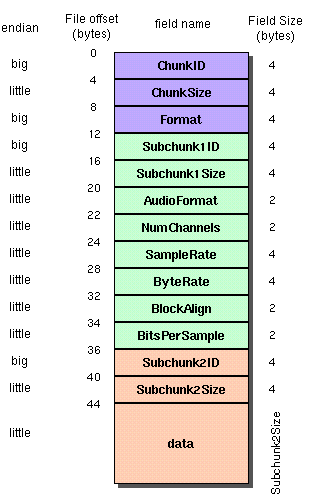
\includegraphics[scale=0.4]{images/wav-header.png}
				\caption{\centering \scriptsize WAV-Header\footnotemark[\thefootnote]}
			\end{figure}
		\end{column}
	\end{columns}
\end{frame}


\begin{frame}{\insertsection}
	\begin{figure}
		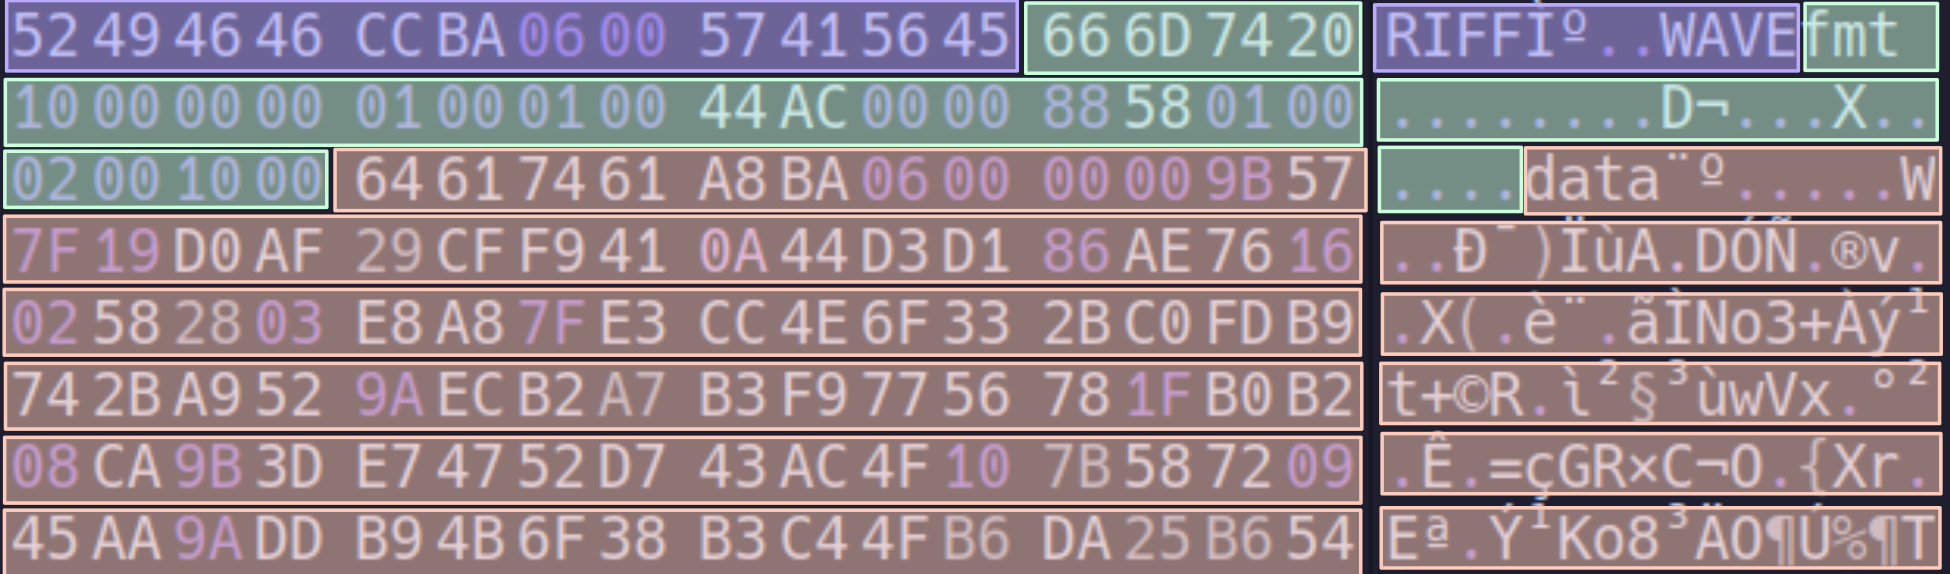
\includegraphics[scale=0.15]{images/wav_hex.png}
		\caption{\centering Ausschnitt einer WAV Datei mit markierten Subchunks,\\dargestellt in einem Hex-Editor}
	\end{figure}
	\begin{itemize}
		\item Abtastrate ist oft $\SI{44.1}{\kilo\hertz}$ \myfootcite{44100Hz},
		\\  Menschen hören Töne im Bereich $\SI{20}{\hertz}-\SI{20}{\kilo\hertz}$ \myfootcite{MenschlicheHoerfrequenz}
		\item Analoges Signal wird durch lineare Pulse Code Modulation (PCM)  in ein digitales Signal umgewandelt (verlustfrei)
	\end{itemize}
\end{frame}